\chapter{Results\index{Results}}


\textsf{In this chapter we present the results of the epxeriments conducted,
reasoning the motivation towards the built models. We also talk about aspects
which were considered but not implemented.}

\section{Overview of Different Models}
The principles behind designing the model are firstly, to accurately account for
biases of various types and secondly, formulation of an efficient low-rank
matrix approximation method. The first principle involves identifying different
biases, like, the user-bias, movie-bias and temporal biases w.r.t users and
movies. These biases are the non-interacting parts between the users and movies,
and they are encapsulated into the baseline predictor. These values are
initially subtracted from all the known ratings. They will be integrated back
into the factor model for the new predicted ratings. We have experimented with
three types of biasing techniques, first without any bias, second, with only
static bias, and third, with temporal movie biases. Moving ahead to the
factorization itself, we start with the SVD technique and owing to the
disadvantages of this method we develop a new factorization technique based on
weighted ALS. Within the ALS algorithm we have two types of initialization
methods, hence leading to ALS-I and ALS-II. The table below shows the various
models built by combining the different biasing and factorizing techniques
mentioned.


\begin{table}
\begin{center}
 
     \begin{tabular}{|c|c|c|c|}
       \hline
        & SVD & ALS-I & ALS-II \\ \hline
       None & Model 1 & Model 6 & Model 7\\        
       $NonTemp_{mu}$ & Model 3 & - & Model 8\\
       $Temp_{mu}$ & Model 2 & - & Model 9\\
       $NonTemp_b$ & - & Model 4 & -\\
       $Temp_b$ & - & Model 5 & -\\ \hline
    \end{tabular}
    \caption{Different Model}     
\end{center}
\end{table}

\subsubsection{SVD}
While using this method, which is [U,S,V]=svds(R,n), where $R$ is the Rating
matrix and $n$ is the rank of the approximatin matrix. We test the models for
different values of $n$, the maximum being $n$=200. The predictions are made in
the following way,

\begingroup
\begin{center}
 

\begin{align*}
 & [U,S,V] = svds(R,200) \\
 & P_u = U(:,1:200); \\
 & Q_i=S(1:l,1:l)*Vt(1:200,:); \\
 & Predicted_rating(i,j)=P_u(i,:)*Q_i(:,j); \\
\end{align*}
\caption{SVD technique}
\end{center}

\endgroup

\subsubsection{ALS-I}
This is the type-I ALS method, where the M matrix is initialized by replacing
the assigning the first row with the mean values of the movies, and filling in
random values at the remaining places. 

\begin{align*}
 & \bold{Step 1.} & Initialize the M matrix, by assigning the means of movies as
the first\\
 &                & row entry, and small random numbers in the remaining
entries. \\
 & \bold{Step 2.} & With this M, solve for U in order to minimize the loss
function.\\
 & \bold{Step 3.} & Now Keep the U matrix from step 2 fixed, and update the M
matrix.\\
 & \bold{Step 4.} & Repeat these iterations until required convergence criteria
is met.\\
\end{align*}

\subsubsection{ALS-II}
This is the type-II ALS method, where the M matrix is initialized by doing an
SVD on the initial rating matrix R, as shown below:

\begingroup
\begin{center}
\begin{align*}
& [U1,S1,V1]=svds(R_Hat_bin,100) \\
& M=S*V' \\
\end{align*}
\caption{SVD Initialization of M}
\end{center}
\endgroup


\begin{align*}
 & \bold{Step 1.} & \left Initialize the M matrix as shown above\\
 &                & \left row entry, and small random numbers in the remaining
entries. \\
 & \bold{Step 2.} & \left With this M, solve for U in order to minimize the loss
function.\\
 & \bold{Step 3.} & \left Now Keep the U matrix from step 2 fixed, and update
the M matrix.\\
 & \bold{Step 4.} & \left Repeat these iterations until required convergence
criteria is met.\\
\end{align*}

\subsubsection{$NonTemp_{mu}$}
This is the non-temporal model with the mean of all movies included in it, it is
given by \\
\begin{equation}
 b_{ui}=\mu+b_u+b_i
\end{equation}
where $b_{ui}$ is the baseline predictor, which encapsulates the non-interacting
parts of user-item relationship, $\mu$ is the mean of all movies which is
$3.6043$, $b_u$ and $b_i$ are the observed deviations from the mean. 

\subsubsection{$Temp_{mu}$}
This is the baseline predictor which involves the tie-changing movie biases,
$b_{i,Bin(t)}$.
\begin{equation}
 b_{ui}=\mu+b_u+b_i+b_{i,Bin(t)}
\end{equation}

\subsubsection{$NonTemp_b$}
This is again non-temporal model, but without the all movie mean $\mu$. This
model is only used in conjuction with the ALS-I method, as in this method the
means is already included into the model during the initialization of M.
\begin{equation}
 b_{ui}=b_u+b_i
\end{equation}

\subsubsection{$Temp_b$}
This is the temporal model without the all movie mean $\mu$, again used for
ALS-I but with time-changing movie biases,
\begin{equation}
 b_{ui}=b_u+b_i+b_{i,Bin(t)}
\end{equation}

\section{Results}
\begin{figure}[h!]
\centering
\subfigure[RMSE for Model 1]{
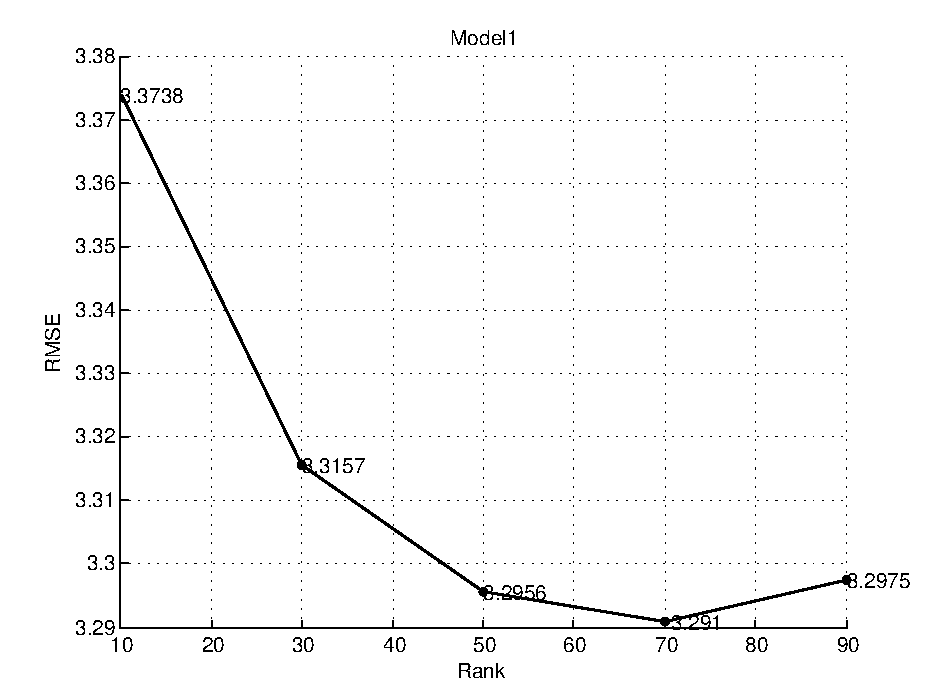
\includegraphics[width=0.45\textwidth]{./Results/plots/model1.pdf}
\label{fig:Model 1}
}
\subfigure[RMSE for Model 2]{
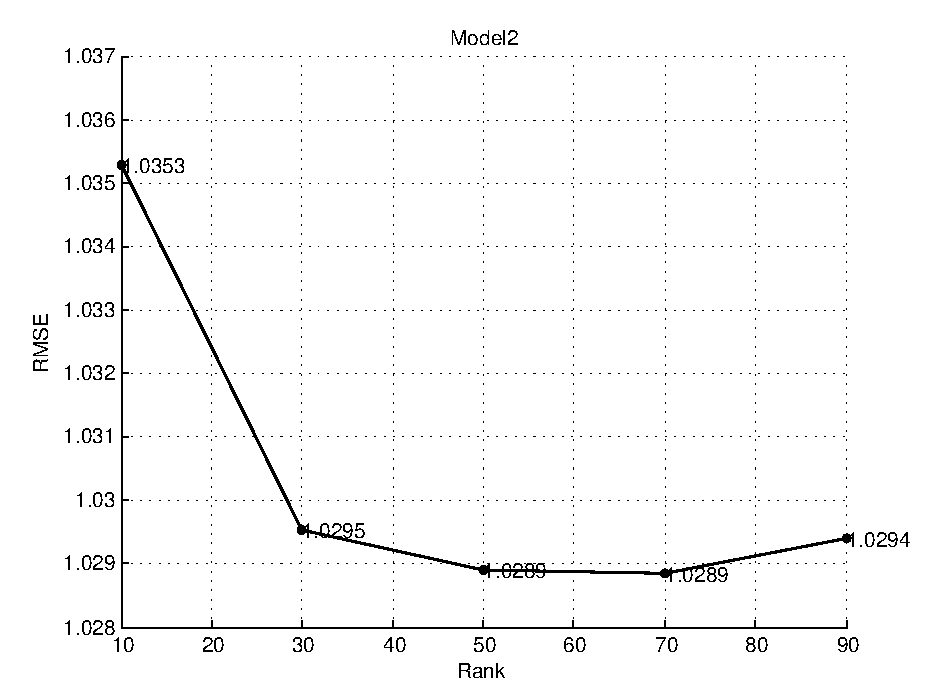
\includegraphics[width=0.45\textwidth]{./Results/plots/model2.pdf}
\label{fig:Model2}
}\\
\subfigure[RMSE for Model 3]{
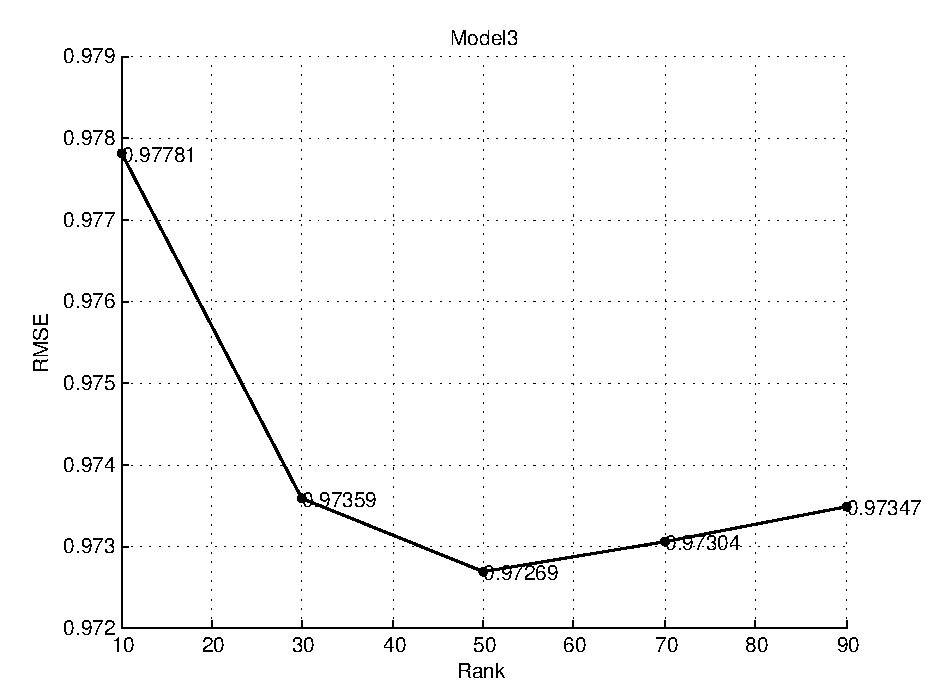
\includegraphics[width=0.45\textwidth]{./Results/plots/model3.pdf}
\label{fig:Model 3}
}
\label{fig:RMSE SVD}
\caption{RMSE: SVD based models}
\end{figure}

In the following figure 5.1, we can see that beyond certain ranks overfitting
occurs. Also we cab observe the improvement in the results by involving the
biases. 

Next we show the results for the ALS based models. Figure 5.2 shows the RMSE of
ALS based models which use the type I initialization technique. 


\begin{figure}[h!]
\centering
\subfigure[RMSE for Model 4 for 30 iterations $N_f=200$]{
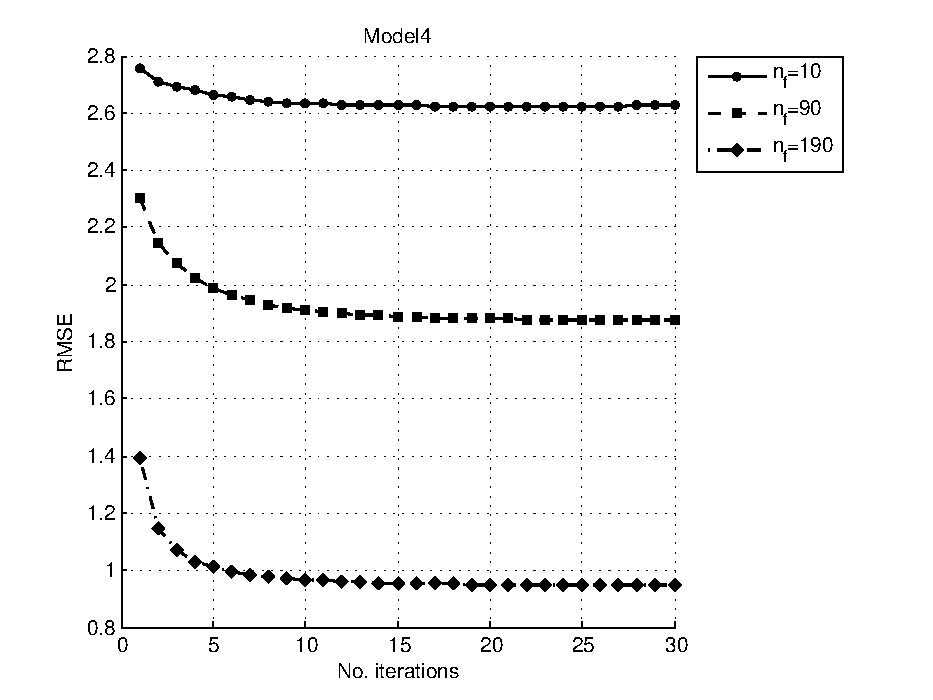
\includegraphics[width=0.45\textwidth]{./Results/plots/model4.pdf}
\label{fig:Model 1}
}
\subfigure[RMSE for Model 4 ]{
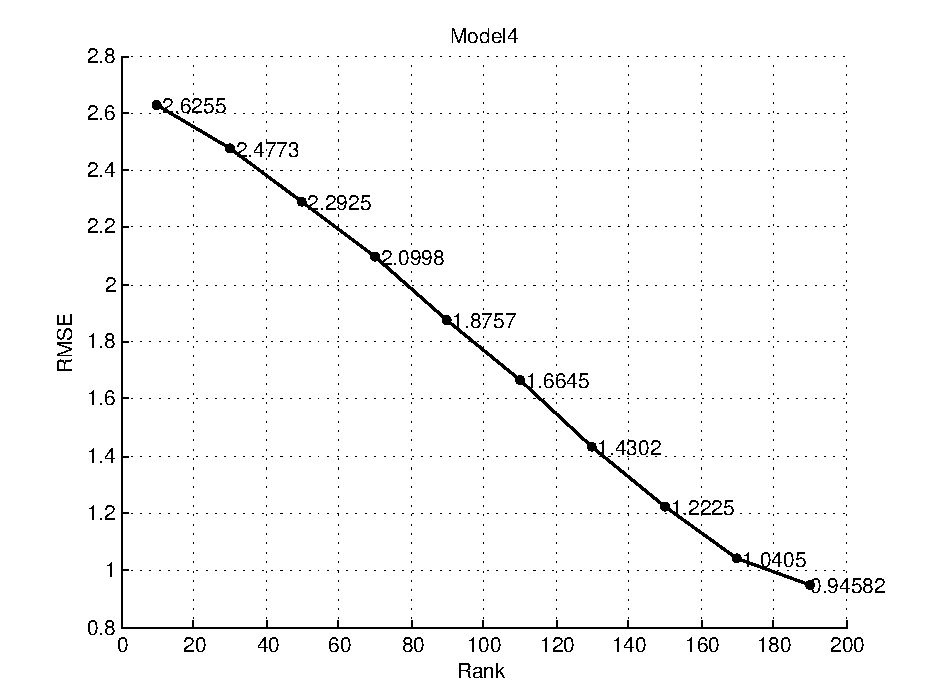
\includegraphics[width=0.45\textwidth]{./Results/plots/model4_1.pdf}
\label{fig:Model2}
}\\
\subfigure[RMSE for Model 5 for 30 iterations $N_f=200$]{
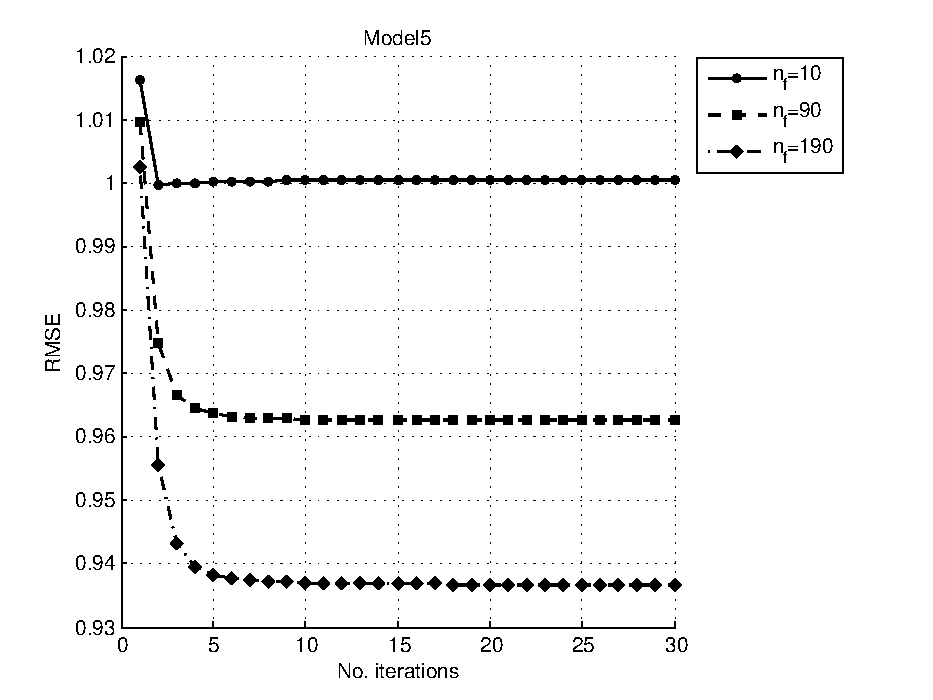
\includegraphics[width=0.45\textwidth]{./Results/plots/model5.pdf}
\label{fig:Model 1}
}
\subfigure[RMSE for Model 5 ]{
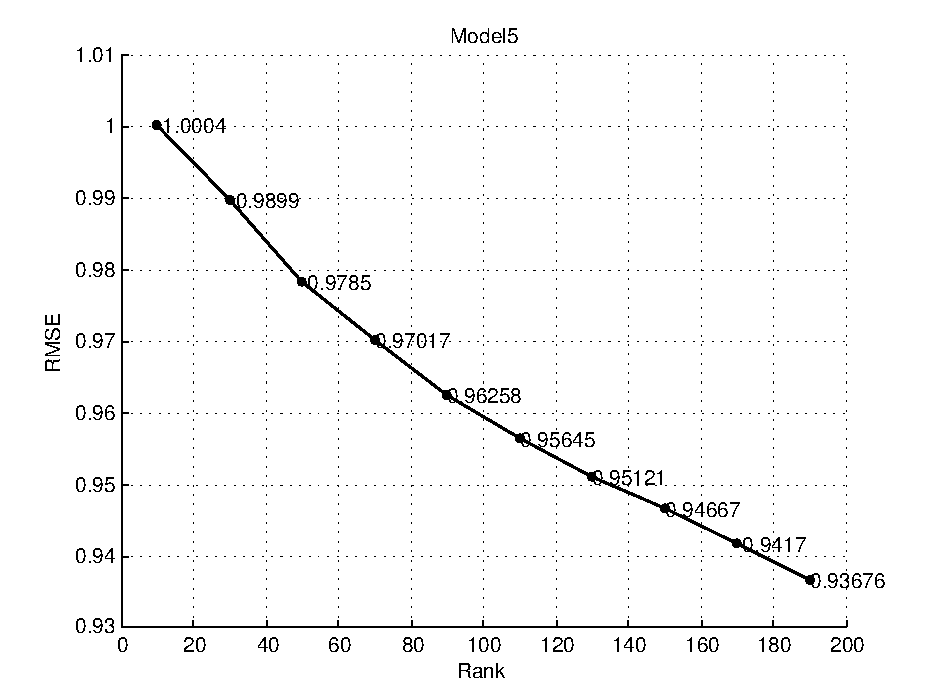
\includegraphics[width=0.45\textwidth]{./Results/plots/model5_1.pdf}
\label{fig:Model2}
}\\
\subfigure[RMSE for Model 6 for 30 iterations $N_f=200$]{
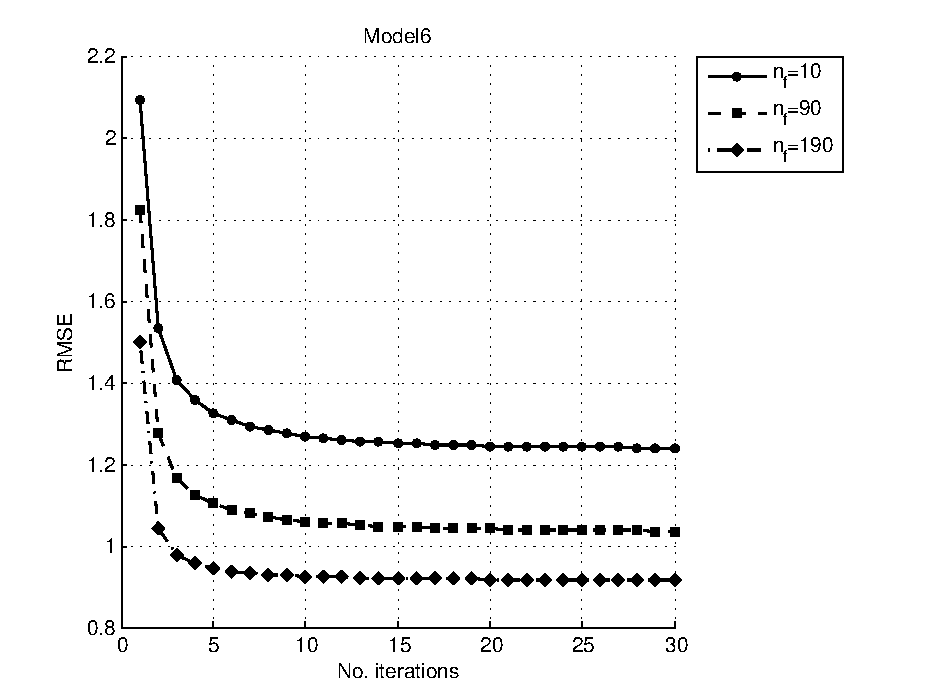
\includegraphics[width=0.45\textwidth]{./Results/plots/model6.pdf}
\label{fig:Model 1}
}
\subfigure[RMSE for Model 6 ]{
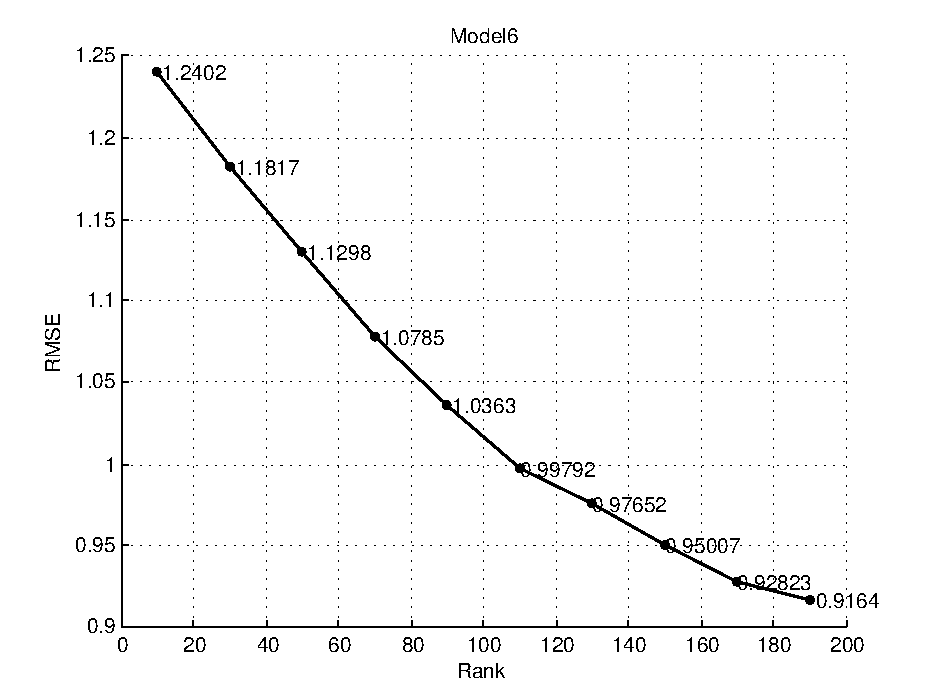
\includegraphics[width=0.45\textwidth]{./Results/plots/model6_1.pdf}
\label{fig:Model2}
}\\
\label{fig:RMSE SVD}
\caption{RMSE: ALS-I based models}
\end{figure}

\begin{figure}[h!]
\centering
\subfigure[RMSE for Model 7 for 30 iterations $N_f=200$]{
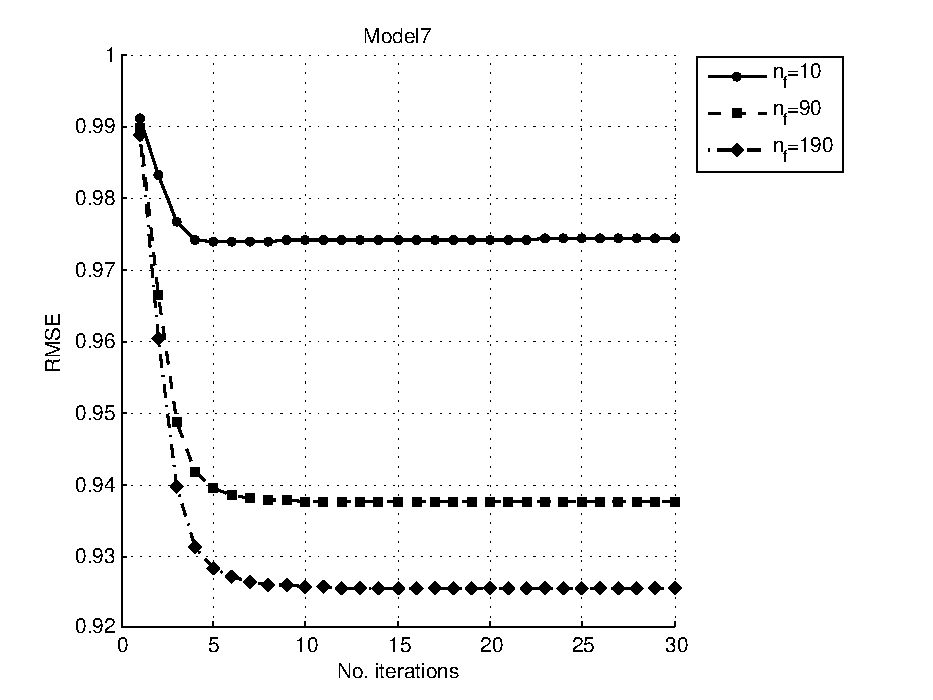
\includegraphics[width=0.45\textwidth]{./Results/plots/model7.pdf}
\label{fig:Model 1}
}
\subfigure[RMSE for Model 7 ]{
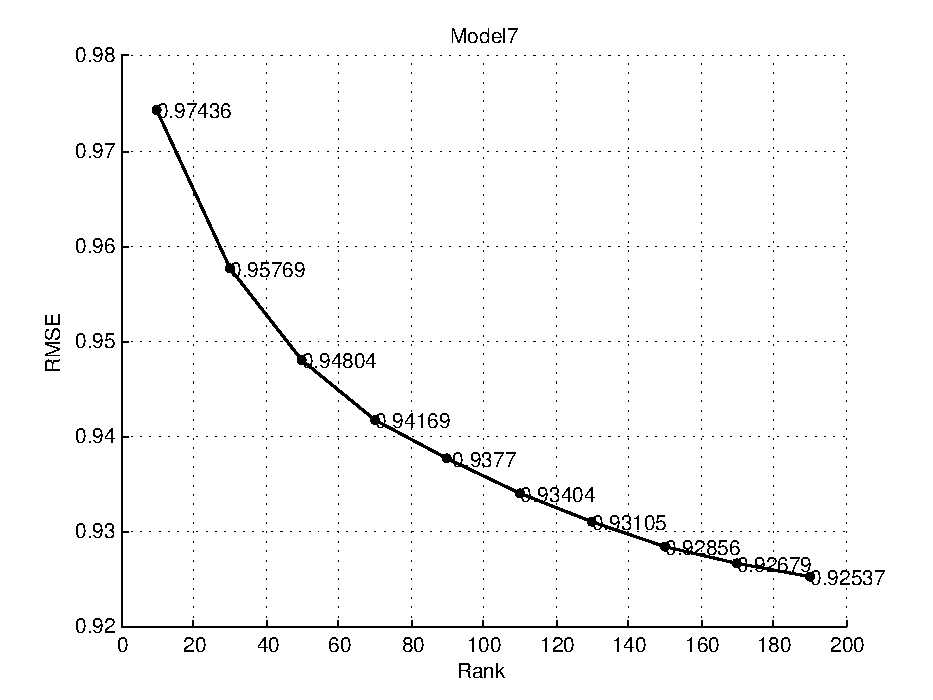
\includegraphics[width=0.45\textwidth]{./Results/plots/model7_1.pdf}
\label{fig:Model2}
}\\
\subfigure[RMSE for Model 8 for 30 iterations $N_f=200$]{
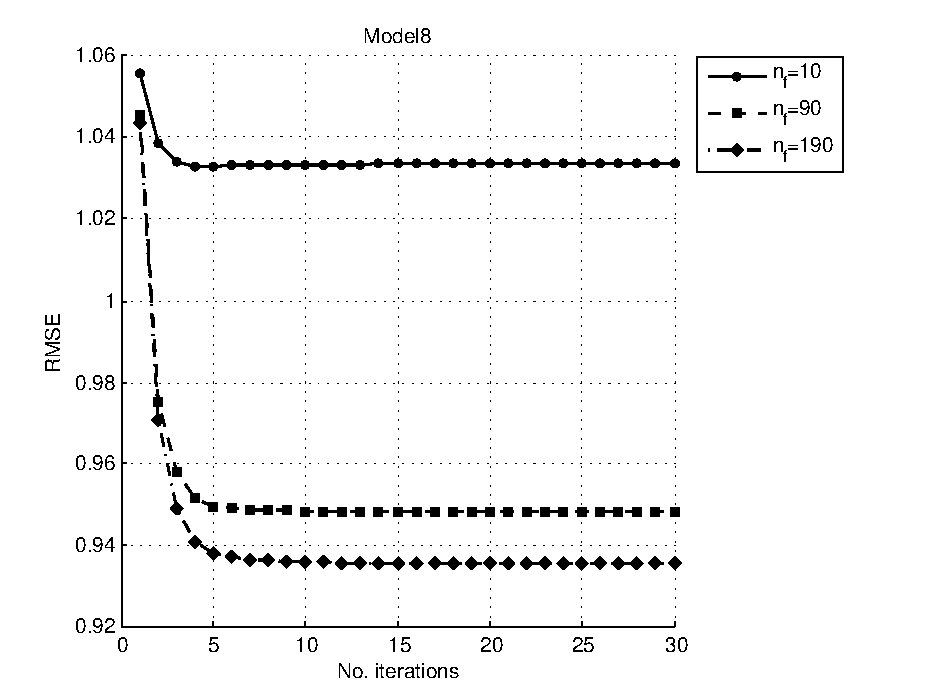
\includegraphics[width=0.45\textwidth]{./Results/plots/model8.pdf}
\label{fig:Model 1}
}
\subfigure[RMSE for Model 8 ]{
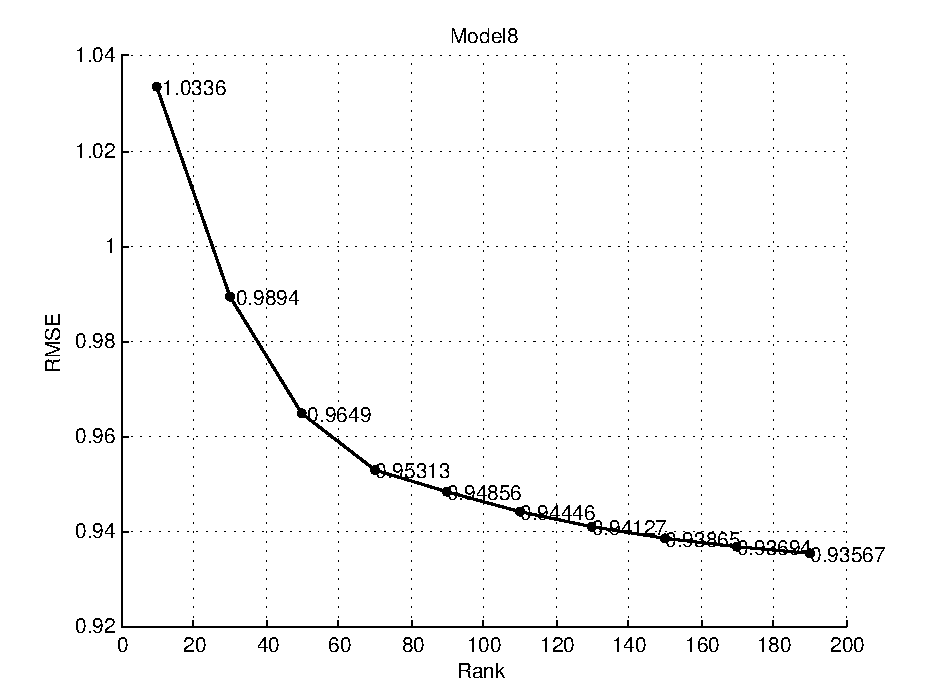
\includegraphics[width=0.45\textwidth]{./Results/plots/model8_1.pdf}
\label{fig:Model2}
}\\
\subfigure[RMSE for Model 9 for 30 iterations $N_f=200$]{
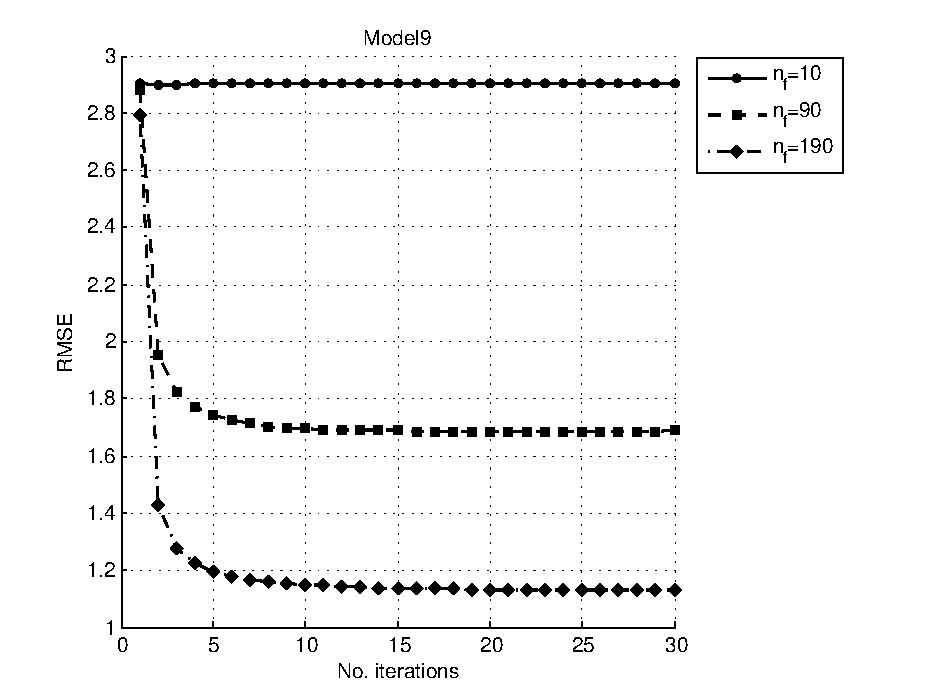
\includegraphics[width=0.45\textwidth]{./Results/plots/model9.pdf}
\label{fig:Model 1}
}
\subfigure[RMSE for Model 9 ]{
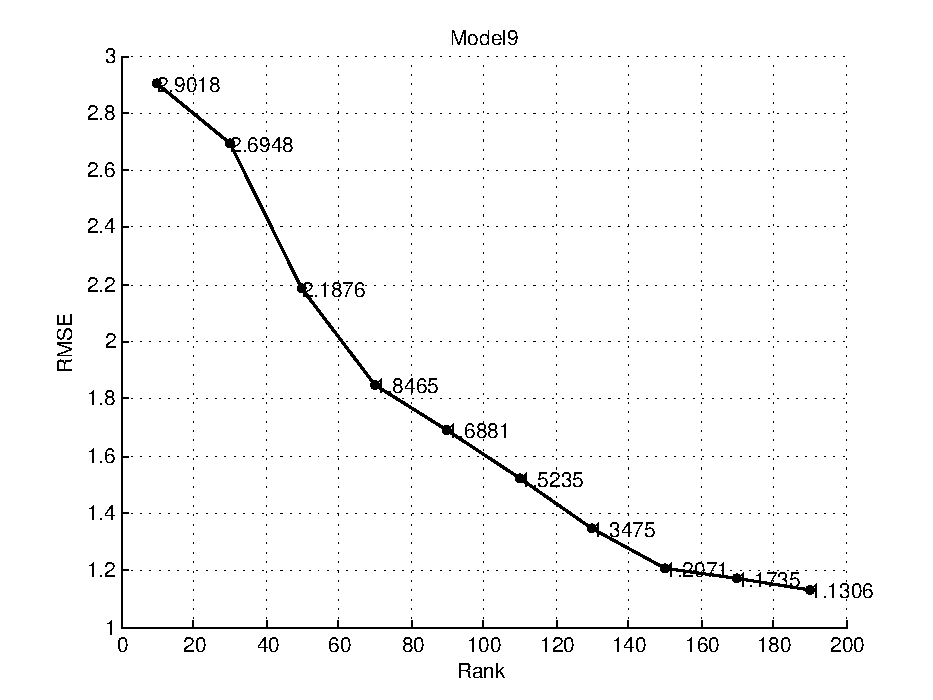
\includegraphics[width=0.45\textwidth]{./Results/plots/model9_1.pdf}
\label{fig:Model2}
}\\
\label{fig:RMSE SVD}
\caption{RMSE: ALS-II based models}
\end{figure}


\section{Future Work}
In this work we have only considered only movie related temporal effects. We
could for future work also include the more complex user realted temporal
effects. The user related temporal dynamics proves to be more comples and more
challenging to model. In a single household different people could be involved
in rating movies, and the mood and temperment of the user is susceptible to more
frequent changes. The user rates on forty different days on average. Apart from
the mood swings, the user could also alter the rating scale over time. We could
for further work consider the various user related effects and incude them into
the model in order to get more accurate predictions. 

Owing to the disadvantages of the sparse SVD of MATLAB, we have used an
alternative method. Instead it is possible to develop a factorization technique
based on SVD, but which is regularised. This approach was suggested initially by
Simon Funk \cite{Paterek_RegSVD}.

We could also aim to improve the prediction accuracy by considering inplicit
feedback. By doing so we can take advantage of additional information about user
preferences. In the current system, where we use only explicit ratings, where
there are users for whom we have very little information, implicit data could
prove to be useful \cite{citeulike:8923836}.








